\documentclass[]{elsarticle} %review=doublespace preprint=single 5p=2 column
%%% Begin My package additions %%%%%%%%%%%%%%%%%%%
\usepackage[hyphens]{url}

  \journal{JEB? RSPB?} % Sets Journal name


\usepackage{lineno} % add
\providecommand{\tightlist}{%
  \setlength{\itemsep}{0pt}\setlength{\parskip}{0pt}}

\bibliographystyle{elsarticle-harv}
\biboptions{sort&compress} % For natbib
\usepackage{graphicx}
\usepackage{booktabs} % book-quality tables
%%%%%%%%%%%%%%%% end my additions to header

\usepackage[T1]{fontenc}
\usepackage{lmodern}
\usepackage{amssymb,amsmath}
\usepackage{ifxetex,ifluatex}
\usepackage{fixltx2e} % provides \textsubscript
% use upquote if available, for straight quotes in verbatim environments
\IfFileExists{upquote.sty}{\usepackage{upquote}}{}
\ifnum 0\ifxetex 1\fi\ifluatex 1\fi=0 % if pdftex
  \usepackage[utf8]{inputenc}
\else % if luatex or xelatex
  \usepackage{fontspec}
  \ifxetex
    \usepackage{xltxtra,xunicode}
  \fi
  \defaultfontfeatures{Mapping=tex-text,Scale=MatchLowercase}
  \newcommand{\euro}{€}
\fi
% use microtype if available
\IfFileExists{microtype.sty}{\usepackage{microtype}}{}
\usepackage{graphicx}
% We will generate all images so they have a width \maxwidth. This means
% that they will get their normal width if they fit onto the page, but
% are scaled down if they would overflow the margins.
\makeatletter
\def\maxwidth{\ifdim\Gin@nat@width>\linewidth\linewidth
\else\Gin@nat@width\fi}
\makeatother
\let\Oldincludegraphics\includegraphics
\renewcommand{\includegraphics}[1]{\Oldincludegraphics[width=\maxwidth]{#1}}
\ifxetex
  \usepackage[setpagesize=false, % page size defined by xetex
              unicode=false, % unicode breaks when used with xetex
              xetex]{hyperref}
\else
  \usepackage[unicode=true]{hyperref}
\fi
\hypersetup{breaklinks=true,
            bookmarks=true,
            pdfauthor={},
            pdftitle={Energetic Consequences of Sonar Exposure for Cetaceans},
            colorlinks=false,
            urlcolor=blue,
            linkcolor=magenta,
            pdfborder={0 0 0}}
\urlstyle{same}  % don't use monospace font for urls

\setcounter{secnumdepth}{0}
% Pandoc toggle for numbering sections (defaults to be off)
\setcounter{secnumdepth}{0}
% Pandoc header
\usepackage{setspace}
\usepackage{lineno}
\usepackage{threeparttable}
\usepackage{float}
\usepackage{pdflscape}



\begin{document}
\begin{frontmatter}

  \title{Energetic Consequences of Sonar Exposure for Cetaceans}
    \author[1]{Max F Czapanskiy\corref{c1}}
   \ead{maxczap@stanford.edu} 
   \cortext[c1]{Corresponding author}
    \author[1]{Matthew S Savoca}
  
  
    \author[1]{Will T Gough}
  
  
    \author[1]{Paolo}
  
  
    \author[1]{Danuta}
  
  
    \author[1]{Jeremy A Goldbogen}
  
  
      \address[1]{Department of Biology, Hopkins Marine Station, Stanford University, 120
Ocean View Boulevard, Pacific Grove, CA 93950, USA}
  
  \begin{abstract}
  The sub-lethal effects of sonar exposure for cetaceans is not well
  enough understood to predict population consequences. To better inform
  conservation planning, we developed a model to predict the energetic
  costs of sonar avoidance behavior. When avoiding sonar sources,
  cetaceans may cease foraging and/or flee the area. We estimate the
  potential energy intake lost to foraging cessation and the additional
  locomotor costs from increased swim speeds.
  
  Although medium-sized cetaceans, especially beaked whales, make up the
  majority of mass strandings associated with naval sonar, our results
  indicate sub-lethal effects cause the most harm to large baleen whales.
  A severe response by a Cuvier's beaked whale (6.5 hour foraging
  cessation and 30 minutes of elevated swim speeds at 4.5 m/s) cost 49\%
  of its daily basal metabolic requirements. Conversely, a moderate
  response by a blue whale (1 hour foraging cessation and 5 minutes of
  elevated swim speeds at 2.5 m/s) cost more than nine times its daily
  basal metabolic requirements. These results may be used to reduce harm
  to endangered cetacean species.
  \end{abstract}
  
 \end{frontmatter}

\doublespacing
\linenumbers

\section{Introduction}\label{introduction}

Naval exercises involving sonar have been linked to mass strandings of
cetaceans worldwide since at least the 1980's (England et al., 2001;
Frantzis, 1998; Jepson et al., 2003; Simmonds and Lopez-Jurado, 1991).
However, the population consequences of sub-lethal effects are not as
well understood. Controlled exposure experiments (CEEs) show that
behavioral responses may include cessation of feeding and/or fleeing the
sonar source at elevated speed (DeRuiter et al., 2017, 2013;
Friedlaender et al., 2016; Goldbogen et al., 2013; Kvadsheim et al.,
2017; Southall et al., 2019; Tyack et al., 2011; Wensveen et al., 2019).
Quantitatively linking these behaviors to demographics requires an
understanding of the impacts on individuals' health (Pirotta et al.,
2018). The mechanism addressed here is reduced energy stores due to lost
foraging opportunities and increased locomotor costs.

The two extant clades of cetaceans differ in their feeding styles.
Toothed whales (odontocetes) are raptorial feeders and locate prey using
echolocation {[}ref?{]}. Baleen whales (mysticetes) are filter feeders
and capture prey by lunging (Goldbogen et al., 2012) or continuous ram
filter feeding (Werth and Potvin, 2016). These feeding styles have
profound effects on feeding rate, energy per feeding event, dive depth,
and body size. Odontocetes feed at higher rates on smaller prey and most
larger odontocetes must dive to extreme depths to find sufficient prey
{[}ref?{]}. Lunge-feeding mysticetes (rorquals) engulf enormous
quantities of prey-laden water, increasing the energy intake per feeding
event but limiting dive depth and duration (Goldbogen et al., 2012).

Feeding rates and the energy obtained per feeding event can be
empirically measured with multi-sensor tags, active acoustics, and
stomach contents {[}jeremy's paper?{]}. The rapid echolocation clicking
(buzzes) preceeding odontocete prey capture events have a kinematic and
acoustic signature that register on tag sensors {[}ref?{]}. Similarly,
rorqual lunges can be identified from an increase in speed followed by a
rapid deceleration, usually associated with high pitch and roll angles
(Cade et al., 2016). Simultaneous prey mapping with tagging efforts
using active acoustics have measured the biomass density of fish and
krill schools targeted by rorquals. The sizes of squid beaks and fish
otoliths \emph{(?)} in odontocete stomach samples are a record of prey
sizes and energy per feeding event.

Empirical estimates of cetacean metabolic rates are logistically
challenging for smaller species and infeasible for larger species.
Oxygen consumption has been measured for captive odontocetes trained to
swim under a metabolic hood using open-flow respirometry, showing that
mass-specific stroke costs are largely size invariant (Williams et al.,
1993, 2017). Whether these metabolic estimates scale to larger
odontocetes or mysticetes is unknown, so other methods of estimating
energy expediture include breathing rates and hydrodynamic models
(Potvin et al., 2012; Sumich, 1983).

Animals swim efficiently by cruising at 1-2 m/s and maintaining a
Strouhal number of 0.25 - 0.3 (Katsufumi et al., 2007; Rohr and Fish,
2004). The Strouhal number is a dimensionless quantity
\(St = \frac{Af}{U}\) where \(A\) is stroke amplitude, \(f\) is stroke
frequency, and \(U\) is swimming speed. Cetacean stroke amplitudes are
approximately one fifth body length {[}ref?{]} so there is a linear
relationship between swimming speed and stroke frequency for animals of
a given body size {[}gough?{]}.

\section{Methods}\label{methods}

We considered the potential energy intake of lost feeding opportunities
and additional energy expenditure from elevated swimming speeds in
modeling the energetic consequences of sonar exposure. The model takes
the form:

\begin{align}
E_{sonar} = P_{in} \times t_d + P_{out}(U_f) \times t_f
\end{align}

Where \(E_{sonar}\) is the energy cost of sonar exposure, \(P_{in}\) is
consumption power (i.e.~rate of energy intake) during undisturbed
foraging, \(t_d\) is the time displaced from foraging, \(P_{out}\) is
flight power (i.e.~increased rate of locomotor costs), \(U_f\) is the
animal's speed during flight, and \(t_f\) is the flight time. \(P_{in}\)
and \(P_{out}\) are species-specific values and \(t_d\), \(U_f\), and
\(t_f\) are dependent on the individual's behavioral response to sonar
exposure.

\subsection{\texorpdfstring{Consumption power
(\(P_{in}\))}{Consumption power (P\_\{in\})}}\label{consumption-power-p_in}

The rate of energy intake is the product of feeding rate (\(r_f\)) and
prey energy per feeding event (\(E_p\)):

\begin{align}
P_{in} = r_f \times E_p
\end{align}

\(r_f\) was calculated as the lunge rate for rorquals and buzz rate for
odontocetes using tag sensors. \(E_p\) was derived using active
acoustics (rorquals) and stomach contents (odontocetes) {[}ref?{]}.

\subsection{\texorpdfstring{Flight power
(\(P_{out}\))}{Flight power (P\_\{out\})}}\label{flight-power-p_out}

The locomotor costs associated with fleeing the sonar source is the
energetic cost of swimming at \(U_f\) relative to the cruising swim
speed. Using the relationship between stroke frequency and swimming
speed and a scaling relationship for mass-specific stroke costs, we
calculate \(P_{out}\) as:

\begin{align}
P_{out}(U_f) = (f_s(U_f) - f_s(U_c)) \times C_L \times m
\end{align}

Where \(f_s\) is a function relating stroke frequency to swimming speed,
\(U_f\) and \(U_c\) are the swimming speeds during the flight response
and cruising, \(C_L\) is the mass-specific locomotor cost of a stroke,
and \(m\) is the animal's mass. Equation (2) assumes, during the flight
response, cetaceans increase swimming speed and stroke frequency, but
the mass-specific locomotor cost of a stroke remains the same regardless
of speed. Although \(C_L\) increases with swimming speed, the scaling
relationships do not hold for larger cetaceans (Williams et al., 2017).
To be conservative, we use the \(C_L\) scaling relationship for cruising
speeds, estimated as \(C_L = 1.46 + 0.0005m\) in
\(J \cdot stroke^{-1} \cdot kg^{-1}\). We chose 1.5 m/s for \(U_c\)
based on size-invariant scaling of cruising speeds (Katsufumi et al.,
2007). Assuming cetaceans maintain a Strouhal number of 0.3 and stroke
amplitude is one fifth body length, stroking frequency as a function of
body length is:

\begin{align}
S_t &= \frac{Af}{U} \notag\\
f &= \frac{1.5U}{L}
\end{align}

\subsection{Case studies}\label{case-studies}

We analyzed tag data from four controlled exposure experiments (CEEs)
and applied the \(E_{sonar}\) model to estimate energetic costs of
observed behavioral responses to sonar exposure {[}BRS ref?{]}. As part
of an on-going behavioral response study to naval sonar, in 2011-2015
\emph{(???)} Blainville's beaked whales (\emph{Mesoplodon
densirostris}), Cuvier's beaked whales (\emph{Ziphius cavirostris}),
northern minke whales (\emph{Balaenoptera acutorostrata}), and blue
whales (\emph{B. musculus}) were tracked with multi-sensor tags and
exposed to mid-frequency active sonar in Southern California. Time
displaced from foraging (\(t_d\)), time in flight (\(t_f\)), and speed
of flight (\(U_f\)) were selected based on tag data. These values should
be considered realistic scenarios, but not the typical or most common
response. Behavioral responses to sonar exposure are highly variable and
seem to depend on received sound level, distance to source, foraging
behavior, and habituation (Southall et al., 2019; Wensveen et al.,
2019).

\subsection{Cross-species comparisons}\label{cross-species-comparisons}

To facilitate comparisons of energetic consequences across body size, we
present \(E_{sonar}\) as 1) the energy cost (\(kJ\)), 2) the
mass-specific energy cost (\(kJ ~~ kg^{-1}\)), and 3) the ratio of
energy cost to daily basal metabolic requirements (\(E_{sonar}:BMR\)).
Kleiber's equation for mammals predicts basal metabolic rate as:
\(BMR = 293.1 m^{0.75} ~~ (kJ/day)\) (Kleiber, 1975). Given the
uncertainty in BMR estimates for large cetaceans and the differences
between basal and active metabolic rates, \(E_{sonar}:BMR\) should be
interpreted as an index of energetic consequence and not an absolute
measure of impact.

\section{Results}\label{results}

\subsection{\texorpdfstring{Consumption power
(\(P_{in}\))}{Consumption power (P\_\{in\})}}\label{consumption-power-p_in-1}

Feeding rates were derived from tag data and tended to decrease with
body size. Rorqual feeding rates ranged from 10.7 to 44.1 lunges/hour
and odontocete feeding rates ranged from 2.5 to 96.8 buzzes/hour (Table
\ref{rf_tbl}).

\begin{table}[t]

\caption{\label{tab:unnamed-chunk-1}Cetacean feeding rates \label{rf_tbl}}
\centering
\begin{threeparttable}
\begin{tabular}{llrr}
\toprule
Group & Species & $r_f$ & N\\
\midrule
Rorqual & \textit{Balaenoptera bonaerensis} & 44.1 & 3\\
Rorqual & \textit{Megaptera novaeangliae} & 17.2 & 6\\
Rorqual & \textit{Balaenoptera physalus} & 13.3 & 3\\
Rorqual & \textit{Balaenoptera musculus} & 10.7 & 11\\
Odontocete & \textit{Phocoena phocoena} & 96.8 & 8\\
Odontocete & \textit{Grampus griseus} & 17.7 & 17\\
Odontocete & \textit{Mesoplodon densirostris} & 13.0 & 14\\
Odontocete & \textit{Globicephala macrorhynchus} & 2.5 & 2\\
Odontocete & \textit{Globicephala melas} & 7.9 & 9\\
Odontocete & \textit{Orcinus orca} & 9.7 & 10\\
Odontocete & \textit{Ziphius cavirostris} & 12.8 & 4\\
Odontocete & \textit{Berardius bairdii} & 4.6 & 1\\
Odontocete & \textit{Physeter macrocephalus} & 12.5 & 36\\
\bottomrule
\end{tabular}
\begin{tablenotes}
\item \textit{Note: } 
\item $r_f$ is lunges/hour (rorquals) or buzzes/hour (odontocetes)
\item Species ordered by size within groups.
\end{tablenotes}
\end{threeparttable}
\end{table}

Prey energy per feeding event was empirically derived from acoustic
backscatter (mysticetes) and stomach samples (odontocetes). Filter
feeders consumed the most energy per feeding event. Generally,
delphinids targeted more energy-rich prey than Ziphids (Fig.
\ref{Ep_fig}).

Modeled consumption power covered four orders of magnitude: from 2.4e3
kJ/hr (\emph{P. phocoena}) to 1.4e7 kJ/hr (\emph{B. musculus}) (Fig.
\ref{Pin_fig}).

\subsection{\texorpdfstring{Flight power
(\(P_{out}\))}{Flight power (P\_\{out\})}}\label{flight-power-p_out-1}

Predicted stroke frequencies at cruising speed decreased with length,
from 1.8 Hz for a 1.22 m \emph{P. phocoena} to 0.09 for a 25 m \emph{B.
musculus} (Fig. \ref{fs_fig}).

Across body sizes, \(P_{out}\) increased linearly with flight speed
(Fig. \ref{Pout_fig}).

\subsection{Case studies}\label{case-studies-1}

We modeled the energetic consequence of sonar exposure for four observed
behavioral responses. The beaked whale (\emph{M. densirostris} and
\emph{Z. cavirostris}) responses were more severe than the rorquals'
(\emph{B. bonaerensis} and \emph{B. musculus}) but the mass-specific
energetic costs and \(E_{sonar}:BMR\) ratio were greater for rorquals
(Table \ref{esonar_tbl}).

\begin{landscape}\begin{table}[t]

\caption{\label{tab:esonar_tbl}Behavioral responses to sonar and estimated energetic consequences of exposure. \label{esonar_tbl}}
\centering
\begin{threeparttable}
\begin{tabular}{lrrrrrrrl}
\toprule
\multicolumn{1}{c}{} & \multicolumn{3}{c}{Behavioral responses} & \multicolumn{5}{c}{Energetic consequences} \\
\cmidrule(l{3pt}r{3pt}){2-4} \cmidrule(l{3pt}r{3pt}){5-9}
Species & $t_d \text{ (min)}$ & $t_f \text{ (min)}$ & $U_f \text{ (m/s)}$ & $E_{out} ~~ (kJ)$ & $E_{in} ~~ (kJ)$ & $E_{sonar} ~~ (kJ)$ & $E_{sonar} ~~ (kJ ~~ kg^{-1})$ & $E_{sonar}:BMR_d$\\
\midrule
M. densirostris & 360 & 30 & 4.5 & 3210 & 20500 & 23700 & 27.5 & 0.509\\
Z. cavirostris & 360 & 30 & 4.5 & 10400 & 46700 & 57000 & 19.7 & 0.492\\
B. bonaerensis & 150 & 60 & 3.5 & 44600 & 949000 & 994000 & 148.0 & 4.58\\
B. musculus & 60 & 5 & 2.5 & 79600 & 14200000 & 14300000 & 153.0 & 9.14\\
\bottomrule
\end{tabular}
\begin{tablenotes}
\item \textit{Note: } 
\item $t_d$ is the time displaced from foraging and $t_f$ is the time fleeing the sonar source at the elevated speed, $U_f$. $E_{out}$ and $E_{in}$ are the energetic costs of increased locomotion and lost feeding, respectively. $E_{sonar}$ is presented as a total cost, as a mass-specific cost, and as a ratio to daily basal metabolic requirements.
\end{tablenotes}
\end{threeparttable}
\end{table}
\end{landscape}

\section{Figures}\label{figures}

\begin{figure}
\centering
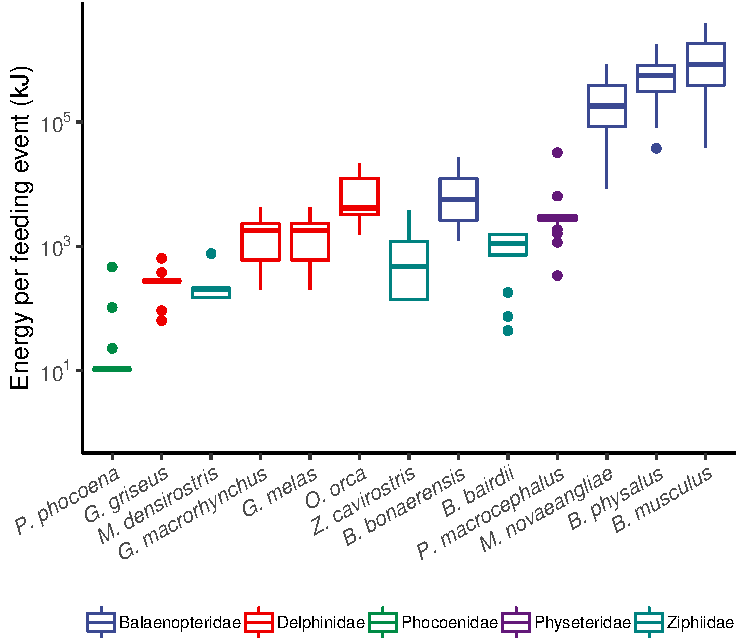
\includegraphics{Sonar_Response_Manuscript_files/figure-latex/Ep_fig-1.pdf}
\caption{Energy per feeding event. Note log scale on y-axis.
\label{Ep_fig}}
\end{figure}

\begin{figure}
\centering
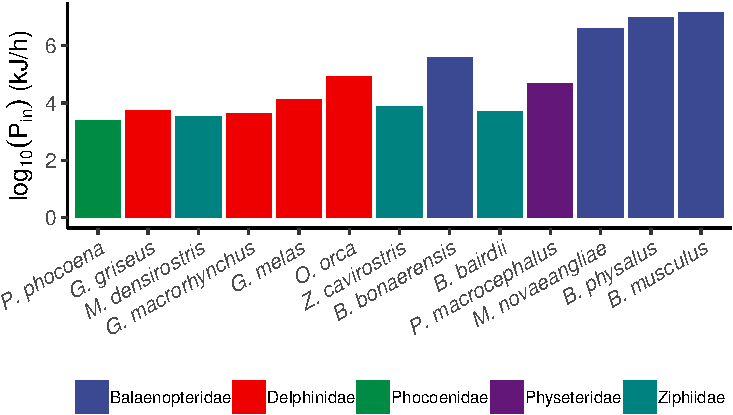
\includegraphics{Sonar_Response_Manuscript_files/figure-latex/Pin_fig-1.pdf}
\caption{Modeled consumption power (\(P_{in}\)). \label{Pin_fig}}
\end{figure}

\begin{figure}
\centering
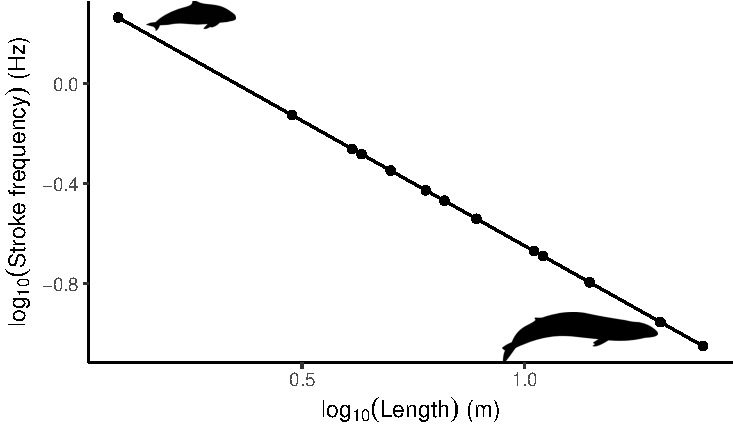
\includegraphics{Sonar_Response_Manuscript_files/figure-latex/fs_fig-1.pdf}
\caption{Predicted cruising speed stroke frequencies (\(f_s\)).
\label{fs_fig}}
\end{figure}

\begin{figure}
\centering
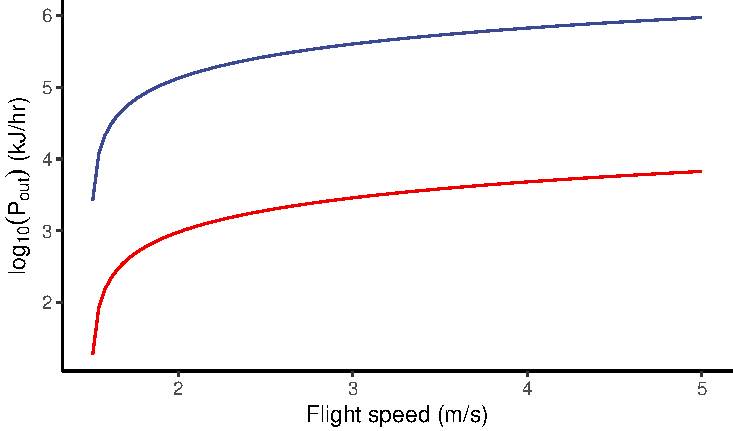
\includegraphics{Sonar_Response_Manuscript_files/figure-latex/Pout_fig-1.pdf}
\caption{Flight power (\(P_{out}\)) by flight speed for
\textit{B. musculus} (blue) and \textit{Z. cavistrostris} (red). Note
log scale on y-axis. \label{Pout_fig}}
\end{figure}

\section*{References}\label{references}
\addcontentsline{toc}{section}{References}

\hypertarget{refs}{}
\hypertarget{ref-cade_kinematic_2016}{}
Cade, D.E., Friedlaender, A.S., Calambokidis, J., Goldbogen, J.A., 2016.
Kinematic diversity in rorqual whale feeding mechanisms. Current Biology
26, 2617--2624. \url{https://doi.org/10.1016/j.cub.2016.07.037}

\hypertarget{ref-deruiter_multivariate_2017}{}
DeRuiter, S.L., Langrock, R., Skirbutas, T., Goldbogen, J.A.,
Calambokidis, J., Friedlaender, A.S., Southall, B.L., 2017. A
multivariate mixed hidden markov model for blue whale behaviour and
responses to sound exposure. The Annals of Applied Statistics 11,
362--392. \url{https://doi.org/10.1214/16-AOAS1008}

\hypertarget{ref-deruiter_first_2013}{}
DeRuiter, S.L., Southall, B.L., Calambokidis, J., Zimmer, W.M.X.,
Sadykova, D., Falcone, E.A., Friedlaender, A.S., Joseph, J.E., Moretti,
D., Schorr, G.S., Thomas, L., Tyack, P.L., 2013. First direct
measurements of behavioural responses by cuvier's beaked whales to
mid-frequency active sonar. Biology Letters 9, 20130223--20130223.
\url{https://doi.org/10.1098/rsbl.2013.0223}

\hypertarget{ref-england_joint_2001}{}
England, G.R., Evans, D., Lautenbacher, C., Morrissey, S., Hogarth, W.,
others, 2001. Joint interim report bahamas marine mammal stranding event
of 15-16 march 2000. US Department of Commerce, US Secretary of the
Navy.

\hypertarget{ref-frantzis_does_1998}{}
Frantzis, A., 1998. Does acoustic testing strand whales? Nature 392,
29--29. \url{https://doi.org/10.1038/32068}

\hypertarget{ref-friedlaender_prey-mediated_2016}{}
Friedlaender, A.S., Hazen, E.L., Goldbogen, J.A., Stimpert, A.K.,
Calambokidis, J., Southall, B.L., 2016. Prey-mediated behavioral
responses of feeding blue whales in controlled sound exposure
experiments. Ecological Applications 26, 1075--1085.
\url{https://doi.org/10.1002/15-0783}

\hypertarget{ref-goldbogen_scaling_2012}{}
Goldbogen, J.A., Calambokidis, J., Croll, D.A., McKenna, M.F., Oleson,
E., Potvin, J., Pyenson, N.D., Schorr, G., Shadwick, R.E., Tershy, B.R.,
2012. Scaling of lunge-feeding performance in rorqual whales:
Mass-specific energy expenditure increases with body size and
progressively limits diving capacity. Functional Ecology 26, 216--226.
\url{https://doi.org/10.1111/j.1365-2435.2011.01905.x}

\hypertarget{ref-goldbogen_blue_2013}{}
Goldbogen, J.A., Southall, B.L., DeRuiter, S.L., Calambokidis, J.,
Friedlaender, A.S., Hazen, E.L., Falcone, E.A., Schorr, G.S., Douglas,
A., Moretti, D.J., Kyburg, C., McKenna, M.F., Tyack, P.L., 2013. Blue
whales respond to simulated mid-frequency military sonar. Proceedings of
the Royal Society B: Biological Sciences 280, 20130657--20130657.
\url{https://doi.org/10.1098/rspb.2013.0657}

\hypertarget{ref-jepson_gas-bubble_2003}{}
Jepson, P.D., Arbelo, M., Deaville, R., Patterson, I.A.P., Castro, P.,
Baker, J.R., Degollada, E., Ross, H.M., Herráez, P., Pocknell, A.M.,
Rodríguez, F., Howie, F.E., Espinosa, A., Reid, R.J., Jaber, J.R.,
Martin, V., Cunningham, A.A., Fernández, A., 2003. Gas-bubble lesions in
stranded cetaceans. Nature 425, 575--576.
\url{https://doi.org/10.1038/425575a}

\hypertarget{ref-katsufumi_stroke_2007}{}
Katsufumi, S., Yutaka, W., Akinori, T., J.O, M.P., Hideji, T., Ryo, K.,
J, P.P., Yves, H., Tomonari, A., Yuuki, W., Yoko, M., P, C.D.,
Charles-André, B., Kagari, A., Masao, A., Phil, T., Ari, S., Yasuhiko,
N., 2007. Stroke frequency, but not swimming speed, is related to body
size in free-ranging seabirds, pinnipeds and cetaceans. Proceedings of
the Royal Society B: Biological Sciences 274, 471--477.
\url{https://doi.org/10.1098/rspb.2006.0005}

\hypertarget{ref-kleiber_fire_1975}{}
Kleiber, M., 1975. The fire of life: An introduction to animal
energetics. Robert E. Krieger, Huntington.

\hypertarget{ref-kvadsheim_avoidance_2017}{}
Kvadsheim, P.H., DeRuiter, S., Sivle, L.D., Goldbogen, J.,
Roland-Hansen, R., Miller, P.J., Lam, F.-P.A., Calambokidis, J.,
Friedlaender, A., Visser, F., Tyack, P.L., Kleivane, L., Southall, B.,
2017. Avoidance responses of minke whales to 1--4 kHz naval sonar.
Marine Pollution Bulletin 121, 60--68.
\url{https://doi.org/10.1016/j.marpolbul.2017.05.037}

\hypertarget{ref-pirotta_understanding_2018}{}
Pirotta, E., Booth, C.G., Costa, D.P., Fleishman, E., Kraus, S.D.,
Lusseau, D., Moretti, D., New, L.F., Schick, R.S., Schwarz, L.K.,
Simmons, S.E., Thomas, L., Tyack, P.L., Weise, M.J., Wells, R.S.,
Harwood, J., 2018. Understanding the population consequences of
disturbance. Ecology and Evolution 8, 9934--9946.
\url{https://doi.org/10.1002/ece3.4458}

\hypertarget{ref-potvin_metabolic_2012}{}
Potvin, J., Goldbogen, J.A., Shadwick, R.E., 2012. Metabolic
expenditures of lunge feeding rorquals across scale: Implications for
the evolution of filter feeding and the limits to maximum body size.
PLOS ONE 7, e44854. \url{https://doi.org/10.1371/journal.pone.0044854}

\hypertarget{ref-rohr_strouhal_2004}{}
Rohr, J.J., Fish, F.E., 2004. Strouhal numbers and optimization of
swimming by odontocete cetaceans. Journal of Experimental Biology 207,
1633--1642. \url{https://doi.org/10.1242/jeb.00948}

\hypertarget{ref-simmonds_whales_1991}{}
Simmonds, M.P., Lopez-Jurado, L.F., 1991. Whales and the military.
Nature 351, 448. \url{https://doi.org/10.1038/351448a0}

\hypertarget{ref-southall_behavioral_2019}{}
Southall, B.L., DeRuiter, S.L., Friedlaender, A., Stimpert, A.K.,
Goldbogen, J.A., Hazen, E., Casey, C., Fregosi, S., Cade, D.E., Allen,
A.N., Harris, C.M., Schorr, G., Moretti, D., Guan, S., Calambokidis, J.,
2019. Behavioral responses of individual blue whales (
\emph{balaenoptera musculus} ) to mid-frequency military sonar. The
Journal of Experimental Biology 222, jeb190637.
\url{https://doi.org/10.1242/jeb.190637}

\hypertarget{ref-sumich_swimming_1983}{}
Sumich, J.L., 1983. Swimming velocities, breathing patterns, and
estimated costs of locomotion in migrating gray whales,
\emph{eschrichtius robustus}. Canadian Journal of Zoology 61, 647--652.
\url{https://doi.org/10.1139/z83-086}

\hypertarget{ref-tyack_beaked_2011}{}
Tyack, P.L., Zimmer, W.M.X., Moretti, D., Southall, B.L., Claridge,
D.E., Durban, J.W., Clark, C.W., D'Amico, A., DiMarzio, N., Jarvis, S.,
McCarthy, E., Morrissey, R., Ward, J., Boyd, I.L., 2011. Beaked whales
respond to simulated and actual navy sonar. PLoS ONE 6, e17009.
\url{https://doi.org/10.1371/journal.pone.0017009}

\hypertarget{ref-wensveen_northern_2019}{}
Wensveen, P.J., Saana, I., Hansen, R.R., Benda-Beckmann, A.M. von,
Kleivane, L., IJsselmuide, S. van, Lam, F.-P.A., Kvadsheim, P.H.,
DeRuiter, S.L., Curé, C., Narazaki, T., Tyack, P.L., Miller, P.J., 2019.
Northern bottlenose whales in a pristine environment respond strongly to
close and distant navy sonar signals. Proceedings of the Royal Society
B: Biological Sciences 286, 20182592.
\url{https://doi.org/10.1098/rspb.2018.2592}

\hypertarget{ref-werth_baleen_2016}{}
Werth, A.J., Potvin, J., 2016. Baleen hydrodynamics and morphology of
cross-flow filtration in balaenid whale suspension feeding. PLOS ONE 11,
e0150106. \url{https://doi.org/10.1371/journal.pone.0150106}

\hypertarget{ref-williams_physiology_1993}{}
Williams, T.M., Friedl, W.A., Haun, J.E., 1993. The physiology of
bottlenose dolphins (tursiops truncatus): Heart rate, metabolic rate and
plasma lactate concentration during exercise. Journal of Experimental
Biology 179, 31--46.

\hypertarget{ref-williams_swimming_2017}{}
Williams, T.M., Kendall, T.L., Richter, B.P., Ribeiro-French, C.R.,
John, J.S., Odell, K.L., Losch, B.A., Feuerbach, D.A., Stamper, M.A.,
2017. Swimming and diving energetics in dolphins: A stroke-by-stroke
analysis for predicting the cost of flight responses in wild
odontocetes. The Journal of Experimental Biology 220, 1135--1145.
\url{https://doi.org/10.1242/jeb.154245}

\end{document}


